\section{比赛故事：从「缺德地图」到 Nav2}

想象你坐在哨兵「脑袋」里要去偷家：需要一张赛场地图、知道自己在哪、算出一条路，边走边躲动态障碍。
这正是导航方向在 RM 中的缩影。算法细节见卷二「导航与 SLAM」；本章只讲\textbf{比赛语义}。

\section{赛场上的模块含义}

对照 Nav2 一类框架，比赛中常见对应关系：

\begin{enumerate}
    \item \textbf{地图}：赛前建图环节得到的静态层 + 比赛中代价地图动态层；
    \item \textbf{定位}：激光雷达 / 里程计 / IMU 等融合（此处「雷达」指 \textbf{LiDAR 传感器}，不是雷达站方向）；
    \item \textbf{全局规划}：在已知地图上找大致路线；
    \item \textbf{局部规划 / 控制}：躲突然出现的障碍，输出速度指令给电控；
    \item \textbf{恢复行为}：卡住后旋转、后退、清代价地图、重规划等；
    \item \textbf{行为树}：编排「规划—跟随—恢复」的比赛逻辑，而不是写死巨型 if-else。
\end{enumerate}

\begin{figure}[H]
    \centering
    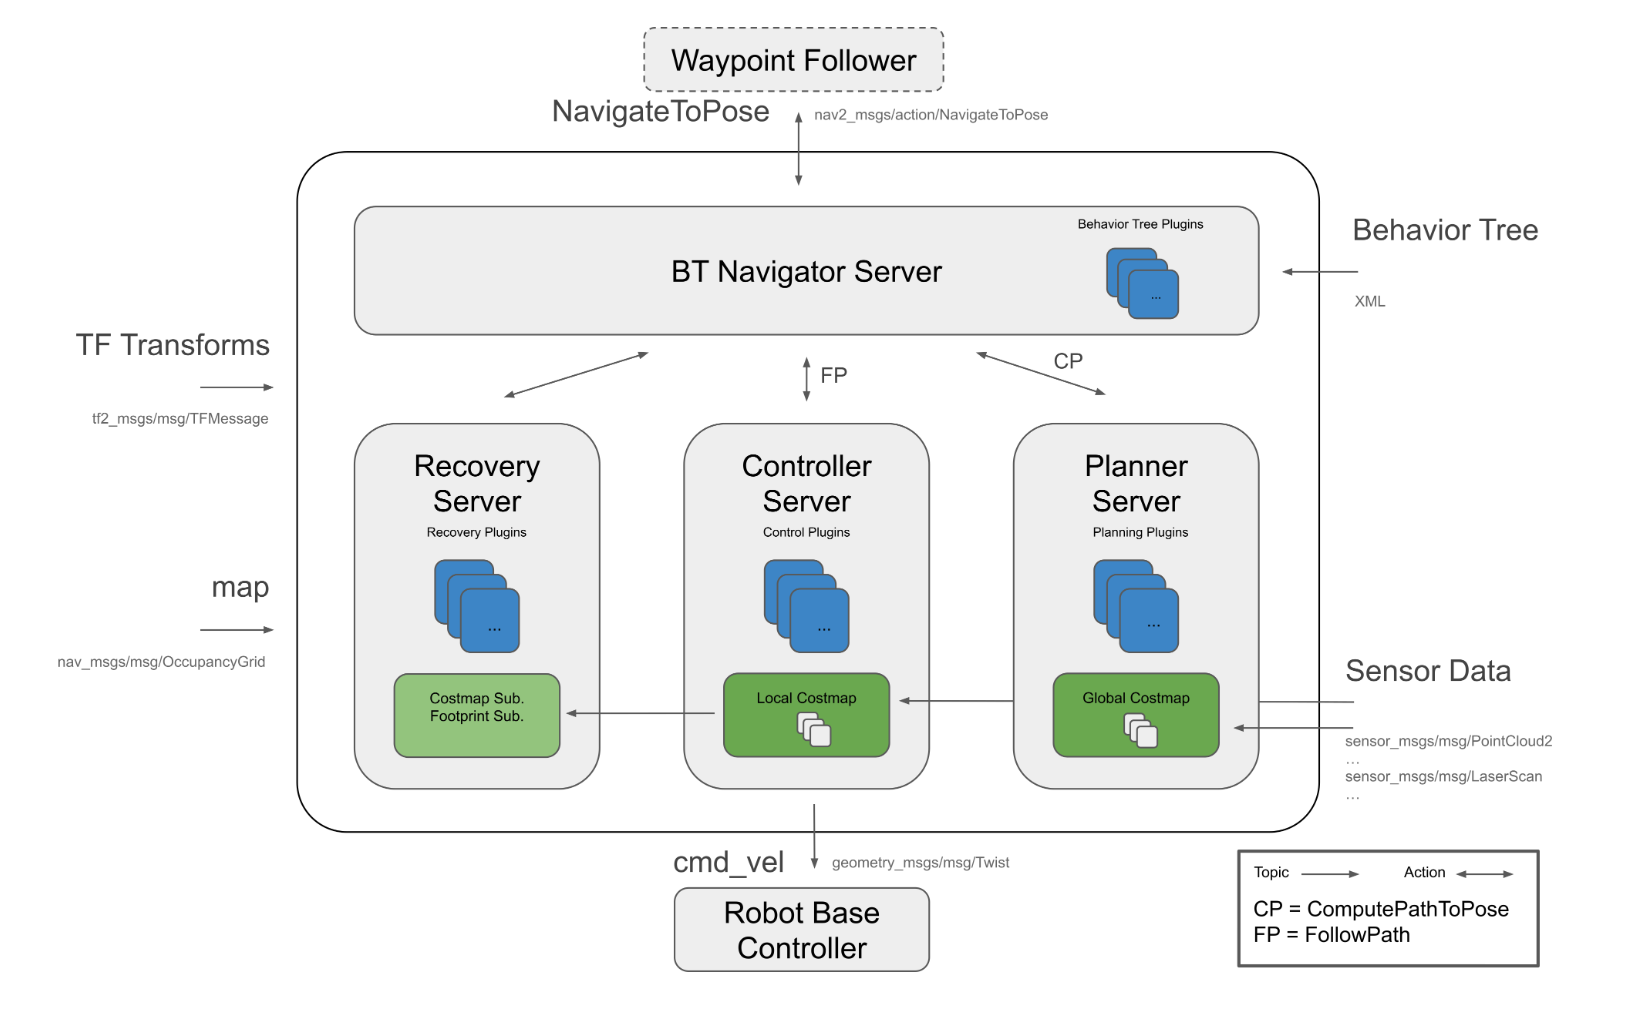
\includegraphics[width=0.85\textwidth]{Nav2导航框架.png}
    \caption{Nav2 导航框架示意（细节回卷二）}
    \label{fig:v3_nav2}
\end{figure}

\section{建图与比赛流程}

\begin{itemize}
    \item 赛前按规则完成哨兵建图，检查噪声黑点、禁行区是否涂正确；
    \item 赛中代价地图必须反映新障碍；膨胀层要按车体尺寸设置，避免「规划成功但车体擦墙」；
    \item 动态障碍（其它机器人等）主要靠局部层与恢复行为，不能只信全局静态图。
\end{itemize}

\section{与雷达、决策的接口}

导航消费「我在哪、路怎么走」；雷达站提供的全场目标位置可辅助战术决策，但\textbf{坐标系统、单位、延时}必须与队内约定一致。
导航不负责高台俯视检测；雷达不负责底盘速度闭环。

\section{故障对照（验收提示）}

| 现象 | 优先怀疑 |
|------|----------|
| 全局路线穿墙 | 地图/膨胀/全局规划器 |
| 有路但贴障发抖 | 局部规划或控制频率 |
| 卡住原地转圈 | 恢复行为配置或代价地图未清 |
| 位姿跳变丢定位 | TF / 定位源融合 |
| 指令有但不走 | 与电控接口或急停 |

验收：对照框图，能把上述现象归到 [1]--[6] 中的一类模块。
